\subsection{Vision}
The image processing algorithm was able to match cards considering shape, shape count and filler. Results of the image processing can be summarised as follows:
\begin{figure}[position = here]
	\begin{centering}
		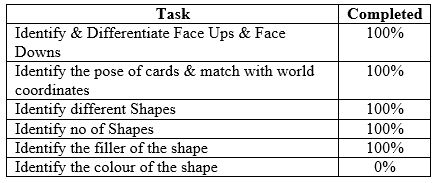
\includegraphics[scale=0.8]{./sachiths_images/image7.png}\\
		\caption[]{\textit{Results Table}}
	\end{centering}
\end{figure}

\textbf{Note:} We were only able to get gray images from the camera as there was a problem with white balancing with the camera driver which we found unable to solve manually. If RGB images were consistently procurable this could have been used to identify the colour of the card simply by checking the dominant colour channels (as RGB is a three-channel format) and would also then be converted into an HSV format image where Hue and Saturation adjustments could be made to resolve shadow problems.

1. Shaded one Rectangle
\begin{figure}[position = here]
	\begin{centering}
		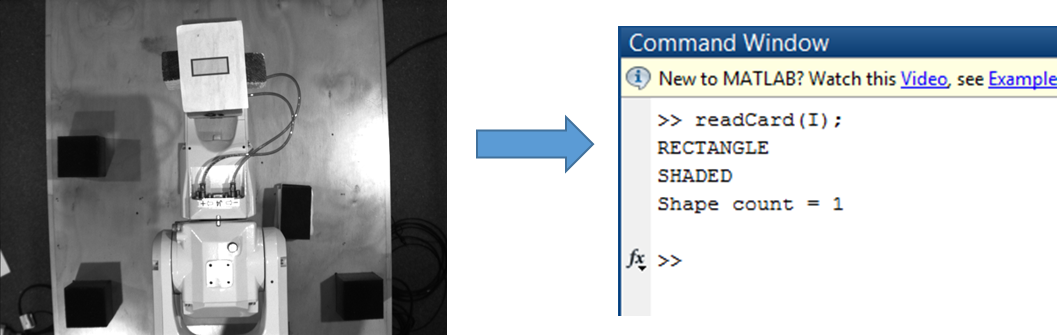
\includegraphics[scale=0.5]{./sachiths_images/image9.png}\\
		\caption[]{\textit{Results for a shaded rectangle}}
	\end{centering}
\end{figure}

2. Block three Rectangles
\begin{figure}[position = here]
	\begin{centering}
		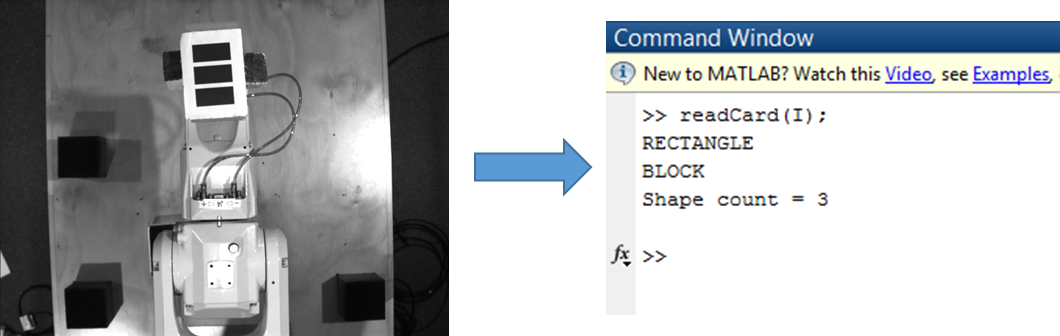
\includegraphics[scale=0.5]{./sachiths_images/image8.png}\\
		\caption[]{\textit{Results for non shaded Triangle}}
	\end{centering}
\end{figure}

3. Shaded one Elipse
\begin{figure}[position = here]
	\begin{centering}
		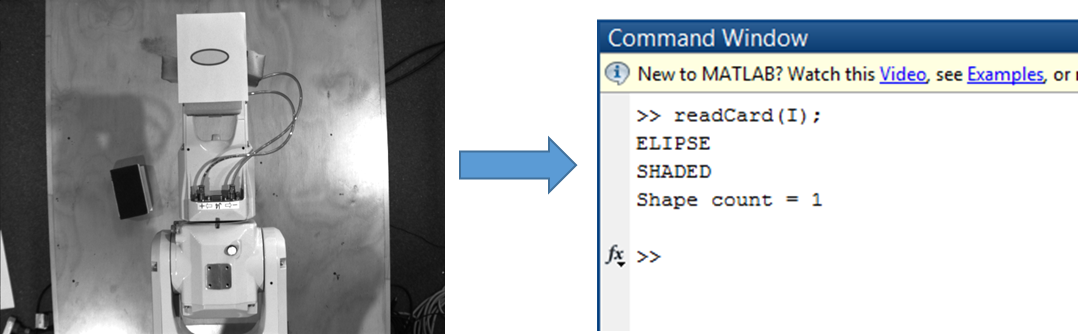
\includegraphics[scale=0.5]{./sachiths_images/image10.png}\\
		\caption[]{\textit{Results for Shaded Elipse}}
	\end{centering}
\end{figure}

